% ============================================================
% CHAPITRE 1 : CADRE GENERAL DU PROJET
% Introduction / organisme / contexte / existant / critique /
% solution / methodologie / conclusion
% ============================================================

\chapter{Cadre général du projet}
\label{chap:cadre-general}
\minitocsection
\newpage

\newcolumntype{P}[1]{>{\raggedright\arraybackslash}p{#1}}

% ------------------------------------------------------------
\section*{Introduction}
\addcontentsline{toc}{section}{Introduction}
% ------------------------------------------------------------

Ce premier chapitre présente le cadre général dans lequel s'inscrit le projet intitulé \textit{« Conception et développement d'un moteur agentique de coaching de vente et d'optimisation dynamique des stocks pour le Retail en temps réel »}. Avant d'aborder les aspects techniques, il est nécessaire de comprendre l'environnement de l'organisme d'accueil, le contexte métier du Retail télécom, les limites des solutions existantes et la démarche méthodologique retenue.

Le chapitre suit une progression classique de rapport d'ingénierie. Nous présentons d'abord l'organisme d'accueil, Ooredoo Tunisie, ses activités et sa clientèle. Nous introduisons ensuite le cadre du projet, la problématique et les objectifs poursuivis. Une étude de l'existant est menée afin d'identifier les solutions déjà utilisées ou disponibles sur le marché et d'en dégager les limites. Sur cette base, nous formulons la solution proposée, puis nous justifions la démarche méthodologique adoptée, fondée sur le processus de référence \textbf{CRISP-DM} (\textit{Cross-Industry Standard Process for Data Mining}), instancié de manière itérative et incrémentale sur douze itérations de deux semaines.

Conformément à la logique du rapport, ce chapitre ne présente pas encore la spécification détaillée des besoins ni les vues d'architecture : les cas d'utilisation et les scénarios relèvent du chapitre~\ref{chap:comprehension-metier}, consacré à la compréhension métier, et l'architecture de la solution du chapitre~\ref{chap:modelisation}, consacré à la modélisation. Le rôle de ce chapitre est de poser une base claire, cohérente et argumentée pour la suite du document.

% ------------------------------------------------------------
\section{Présentation de l'organisme d'accueil}
% ------------------------------------------------------------

\subsection{Présentation d'Ooredoo Tunisie}

Ooredoo Tunisie, anciennement \textit{Tunisiana}, est l'un des principaux opérateurs de télécommunications en Tunisie. L'entreprise évolue dans un secteur stratégique caractérisé par une forte concurrence, une évolution rapide des technologies et une demande croissante en services numériques. Elle propose des services de téléphonie mobile, d'internet fixe et mobile, de fibre optique, de connectivité et de services digitaux, à destination des particuliers comme des professionnels.

Depuis son implantation sur le marché tunisien, Ooredoo Tunisie a renforcé son positionnement en misant sur l'innovation, la proximité client, la diversification des offres et la qualité de service. L'entreprise s'appuie sur un réseau de points de vente, de canaux digitaux et de partenaires de distribution qui lui assure une présence commerciale étendue sur le territoire.

Dans un environnement télécom en mutation, l'exploitation intelligente des données devient un levier essentiel pour améliorer la performance commerciale, anticiper les besoins des clients, garantir la disponibilité des produits et soutenir les équipes terrain. C'est dans cette dynamique que s'inscrit le présent projet, orienté vers l'utilisation de l'intelligence artificielle agentique pour assister les conseillers de vente et les managers Retail.

La figure~\ref{fig:ooredoo-logo-chap1} présente l'identité visuelle de l'entreprise.

\begin{figure}[H]
    \centering
    
\includegraphics[width=0.32\textwidth]{img/ooredoo_logo.png}
    \caption{Logo de l'entreprise Ooredoo Tunisie}
    \label{fig:ooredoo-logo-chap1}
\end{figure}

\subsection{Activités principales d'Ooredoo Tunisie}

Les activités d'Ooredoo Tunisie couvrent quatre familles de services complémentaires.

\begin{itemize}[label=--]
    \item \textbf{Services mobiles} : offres prépayées et postpayées, appels, SMS, internet mobile, recharges, forfaits data et services associés.
    \item \textbf{Services fixes et haut débit} : internet fixe, fibre optique, box 4G/5G et solutions de connectivité résidentielle.
    \item \textbf{Services digitaux} : applications mobiles, services à valeur ajoutée, contenus numériques, plateformes de \textit{self-care} et canaux digitaux de relation client.
    \item \textbf{Services entreprises} : offres B2B, connectivité professionnelle, solutions réseau, services cloud, sécurité et accompagnement digital.
\end{itemize}

Dans le cadre du présent projet, l'attention est portée sur l'activité \textbf{Retail}, c'est-à-dire les interactions entre l'entreprise, ses points de vente, ses conseillers et ses clients finaux. Ce périmètre est déterminant : il constitue un point de contact direct avec le client et un lieu où les décisions commerciales doivent être prises rapidement, avec une information partielle et sous contrainte de temps.

\subsection{La clientèle d'Ooredoo Tunisie}

La clientèle d'Ooredoo Tunisie se segmente en deux grandes catégories :

\begin{itemize}[label=--]
    \item la clientèle \textbf{B2C}, composée de particuliers utilisant les services mobiles, data, fixes, fibre ou box ;
    \item la clientèle \textbf{B2B}, composée d'entreprises, d'institutions et de professionnels nécessitant des solutions de connectivité et des services adaptés à leurs activités.
\end{itemize}

Le projet se concentre sur le segment \textbf{B2C Retail}, car il concerne les ventes réalisées en boutique, les interactions avec les conseillers, les niveaux de stock en point de vente et les objectifs commerciaux quotidiens. Dans ce contexte, la qualité du conseil, la disponibilité produit et la réactivité du vendeur déterminent directement la conversion commerciale et la satisfaction client.

\subsection{Valeurs et culture de service}

Les valeurs d'Ooredoo Tunisie reposent notamment sur la proximité, l'engagement, la confiance, la collaboration et l'amélioration continue. Ces valeurs ont une conséquence directe sur la conception du système : le moteur de coaching visé ne doit pas seulement produire une décision technique, il doit produire un conseil compréhensible, justifié et exploitable par les équipes terrain, que l'utilisateur reste libre d'accepter, de modifier ou de rejeter.

La figure~\ref{fig:ooredoo-values-chap1} illustre les valeurs sur lesquelles l'entreprise fonde sa relation client.

\begin{figure}[H]
    \centering
    
\includegraphics[width=0.88\textwidth]{img/ooredoo_values.png}
    \caption{Valeurs d'Ooredoo Tunisie}
    \label{fig:ooredoo-values-chap1}
\end{figure}

\subsection{Organisation générale de l'entreprise}

L'organisation d'Ooredoo Tunisie repose sur plusieurs directions complémentaires : direction générale, direction commerciale, direction marketing, direction technique, direction des systèmes d'information, direction financière, direction des ressources humaines, direction juridique et fonctions support. Cette organisation reflète la complexité d'un opérateur télécom, qui doit simultanément gérer son infrastructure réseau, piloter son activité commerciale, maintenir ses systèmes d'information et répondre aux attentes de ses clients.

Le projet s'inscrit dans une logique transversale : il mobilise des données et des besoins issus de plusieurs périmètres — ventes, stocks, objectifs commerciaux, connaissance métier, reporting et pilotage opérationnel.

La figure~\ref{fig:ooredoo-organigramme-chap1} présente l'organisation générale de l'entreprise.

\begin{figure}[H]
    \centering
    
\includegraphics[width=0.93\textwidth]{img/ooredoo_organigramme.png}
    \caption{Organisation générale d'Ooredoo Tunisie}
    \label{fig:ooredoo-organigramme-chap1}
\end{figure}

\subsection{Direction concernée par le projet}

La Direction des Systèmes d'Information joue un rôle central dans la transformation digitale de l'entreprise. Elle assure l'intégration des applications, la gestion des bases de données, la fiabilité des flux métier, la sécurité des systèmes et l'évolution des outils décisionnels. Dans le cadre de ce projet, son rôle est essentiel : la plateforme à concevoir nécessite l'accès à des données commerciales et opérationnelles ainsi qu'une intégration maîtrisée dans l'environnement existant.

Le projet touche également les équipes Retail : responsables de boutique, managers commerciaux et acteurs impliqués dans la gestion des stocks. Cette dimension transversale impose de concevoir une solution compréhensible par les utilisateurs métier tout en restant techniquement robuste.

La figure~\ref{fig:ooredoo-direction-technique-chap1} situe la direction concernée par le projet au sein de cette organisation.

\begin{figure}[H]
    \centering
    
\includegraphics[width=0.9\textwidth]{img/ooredoo_direction_technique.png}
    \caption{Positionnement de la direction technique au sein d'Ooredoo Tunisie}
    \label{fig:ooredoo-direction-technique-chap1}
\end{figure}

% ------------------------------------------------------------
\section{Contexte général du projet}
% ------------------------------------------------------------

\subsection{Cadre du projet}

Dans les environnements Retail télécom, la performance commerciale d'un point de vente dépend de facteurs nombreux et hétérogènes : le trafic en boutique, le niveau d'atteinte de l'objectif journalier, la disponibilité des produits, la pertinence de l'offre proposée, l'expérience du conseiller, le moment de la journée, ainsi que des signaux externes tels que les événements locaux, les promotions, les périodes de forte affluence ou les conditions météorologiques.

Le conseiller de vente doit prendre, en quelques secondes et face au client, des décisions opérationnelles : quel produit recommander, quelle offre pousser, quel argumentaire employer, quel produit éviter parce qu'il est en rupture, quel client accompagner en priorité et quand alerter son responsable. Le manager, de son côté, doit arbitrer : quelles boutiques nécessitent une intervention, quels réapprovisionnements engager, quelles recommandations valider. Ces décisions sont aujourd'hui prises à partir d'indicateurs fragmentés, de règles fixes ou de l'expérience individuelle.

Le projet s'inscrit dans ce contexte. Il vise à transformer les données Retail disponibles — historique de ventes à granularité journalière et horaire, niveaux de stock par référence, objectifs commerciaux, catalogue d'offres, contexte externe — en recommandations actionnables et contextualisées. L'objectif n'est donc pas de produire un tableau de bord supplémentaire ni une simple prévision, mais de fournir une assistance décisionnelle temps réel qui améliore la réactivité commerciale et la gestion dynamique des stocks.

\subsection{Problématique}

Les outils traditionnels de suivi commercial permettent de visualiser la performance, mais ils restent limités lorsqu'il s'agit de recommander une action au bon moment. Les données de ventes, de stock, d'objectifs et de contexte existent, mais elles sont rarement exploitées ensemble dans une logique proactive : un écart de chiffre d'affaires est constaté en fin de journée, alors qu'il aurait pu être détecté et corrigé dès la deuxième heure ; une rupture est constatée lorsque le client la subit, alors que la couverture de stock la rendait prévisible plusieurs jours à l'avance.

La problématique du projet peut donc être formulée comme suit :

\begin{quote}
\textit{Comment concevoir et développer un moteur intelligent capable d'exploiter les données Retail en temps réel afin de générer des recommandations commerciales et logistiques explicables, actionnables et adaptées au contexte des conseillers et des managers d'Ooredoo Tunisie ?}
\end{quote}

Cette problématique se décompose en cinq questions opérationnelles :

\begin{itemize}[label=--]
    \item comment détecter, en cours de journée, un retard sur objectif ou un risque de rupture, et non a posteriori ?
    \item comment expliquer un écart de performance à partir du contexte interne et externe plutôt que de le constater ?
    \item comment recommander une action pertinente au conseiller sans alourdir son travail ni interrompre la relation client ?
    \item comment aider le manager à prioriser les produits, les conseillers et les réapprovisionnements nécessitant une intervention ?
    \item comment garantir la fiabilité des recommandations produites par un modèle de langage et capitaliser sur les retours des utilisateurs pour les améliorer ?
\end{itemize}

\subsection{Objectifs du projet}

L'objectif général est de concevoir et de développer un moteur agentique de coaching de vente et d'optimisation dynamique des stocks pour le Retail en temps réel. Il se décline en objectifs spécifiques :

\begin{itemize}[label=--]
    \item centraliser et fiabiliser les données Retail nécessaires à la décision (ventes, stocks, objectifs, offres, contexte) ;
    \item analyser en continu les écarts entre ventes réalisées, prévisions et objectifs, à l'échelle de la journée et de l'heure ;
    \item détecter les risques liés aux stocks — rupture, couverture insuffisante, surstock — et les hiérarchiser ;
    \item enrichir l'analyse avec des signaux contextuels pertinents : promotions, événements locaux, jours fériés, météo ;
    \item exploiter les règles métier, les catalogues d'offres et les scripts commerciaux au moyen d'une base de connaissances interrogeable ;
    \item générer des recommandations courtes, justifiées et directement utilisables par le conseiller et par le manager ;
    \item soumettre les décisions engageantes à une validation humaine et conserver la trace des arbitrages ;
    \item évaluer la qualité des recommandations et intégrer le retour des utilisateurs pour l'améliorer dans le temps.
\end{itemize}

\subsection{Périmètre retenu}

Le périmètre fonctionnel couvre deux domaines complémentaires, traités par le même système : le domaine \textbf{Ventes} (analyse de la performance, prévision, coaching commercial) et le domaine \textbf{Stocks} (analyse d'inventaire, prévision de demande, décision de réapprovisionnement et cycle de commande). Certains sujets ont été volontairement exclus : l'interface multilingue, une application mobile native, l'intégration à un ERP de production et l'entraînement spécifique d'un modèle de langage propriétaire. Ces arbitrages sont détaillés au chapitre~\ref{chap:comprehension-metier}.

% ------------------------------------------------------------
\section{Étude de l'existant}
% ------------------------------------------------------------

\subsection{Existant interne}

Dans le fonctionnement classique d'un point de vente Retail, le pilotage repose sur des tableaux de bord, des rapports périodiques, des objectifs commerciaux et des échanges entre conseillers, responsables de boutique et managers. Ces outils donnent une vision globale de la performance, mais ils demeurent majoritairement descriptifs.

L'existant interne présente les caractéristiques suivantes :

\begin{itemize}[label=--]
    \item les ventes sont suivies au travers d'indicateurs agrégés : chiffre d'affaires, volumes vendus, produits activés, taux d'atteinte de l'objectif ;
    \item les stocks sont suivis à partir de niveaux disponibles, de seuils critiques et de mouvements d'alimentation, sans lien systématique avec la demande prévue ;
    \item les analyses sont produites par période, boutique, produit ou conseiller, généralement après la clôture de la journée ;
    \item les recommandations commerciales reposent sur l'expérience métier, les consignes managériales ou les campagnes en cours ;
    \item le retour terrain — ce que le conseiller a réellement fait de la consigne — n'est pas capitalisé.
\end{itemize}

Les données existent donc, mais elles ne sont pas mobilisées ensemble ni au moment où la décision se prend. Le besoin ne consiste pas à ajouter un tableau de bord supplémentaire, mais à transformer ces données en conseils opérationnels contextualisés.

\subsection{Solutions existantes sur le marché}

Plusieurs familles de solutions couvrent partiellement les besoins visés. Elles relèvent du CRM augmenté par l'IA, du pilotage décisionnel, de la planification de la chaîne d'approvisionnement et de l'optimisation des stocks.

\begin{itemize}[label=--]
    \item \textbf{CRM intelligents} (Salesforce avec \textit{Einstein}/\textit{Agentforce}, Microsoft Dynamics~365 avec \textit{Copilot}, Zoho~CRM avec \textit{Zia}) : ils assistent les équipes commerciales dans la qualification des opportunités, la priorisation des actions, la rédaction et le compte rendu.
    \item \textbf{Plateformes de Business Intelligence} (Microsoft Power~BI, Tableau, Qlik) : elles offrent des tableaux de bord, des indicateurs et des alertes sur seuils.
    \item \textbf{Solutions de planification et d'optimisation des stocks} (SAP~IBP, Blue~Yonder, RELEX~Solutions, o9~Solutions) : elles prévoient la demande, calculent les stocks de sécurité et recommandent des réapprovisionnements à l'échelle du réseau.
    \item \textbf{Outils d'\textit{inventory advisor}} intégrés aux ERP et aux systèmes de gestion commerciale : ils détectent les déséquilibres de stock et proposent des actions de rééquilibrage.
    \item \textbf{Assistants génériques fondés sur les modèles de langage} (ChatGPT, Copilot et équivalents) : ils génèrent du texte et répondent à des questions ouvertes, sans accès natif aux données ni garantie de conformité métier.
\end{itemize}

Ces solutions apportent des réponses réelles, mais chacune sur un périmètre isolé : la vente, le stock, le reporting ou la relation client. Peu d'entre elles combinent simultanément le coaching commercial en boutique, la prévision, le contexte local, la disponibilité produit et la génération de recommandations explicables destinées au conseiller.

\subsection{Synthèse comparative de l'existant}

Le tableau~\ref{tab:comparaison-existant-chap1} synthétise les catégories étudiées et leur positionnement par rapport au besoin exprimé.

\begin{longtable}{|P{3.0cm}|P{4.0cm}|P{4.2cm}|P{3.4cm}|}
\hline
\rowcolor{red!75}
\textcolor{white}{\textbf{Catégorie}} &
\textcolor{white}{\textbf{Apports principaux}} &
\textcolor{white}{\textbf{Limites observées}} &
\textcolor{white}{\textbf{Écart avec notre besoin}} \\
\hline
\endhead
\hline
\endfoot
\hline
\endlastfoot
CRM intelligent \newline \small (Einstein, Copilot, Zia) & Suivi commercial, priorisation des opportunités, assistance à la rédaction & Orienté cycle de vente B2B et pipeline ; peu adapté au rythme d'une boutique & N'assiste pas le conseiller pendant la vente, à l'échelle de l'heure \\
\hline
Business Intelligence \newline \small (Power BI, Tableau, Qlik) & Tableaux de bord, indicateurs, alertes sur seuils & Approche descriptive : constate l'écart sans proposer l'action & Ne transforme pas l'écart en argumentaire ni en décision \\
\hline
Planification de la demande \newline \small (SAP IBP, Blue Yonder, RELEX) & Prévision de la demande, stock de sécurité, réapprovisionnement réseau & Orienté entrepôt et cycle hebdomadaire ; coût et intégration lourds & Ne relie pas le stock à l'objectif commercial du jour en boutique \\
\hline
Inventory advisor \newline \small (modules ERP) & Détection des ruptures et surstocks, propositions de commande & Centré sur la disponibilité produit, sans dimension commerciale & Ne couvre ni l'argumentaire de vente ni le contexte client \\
\hline
Assistants LLM génériques & Génération de texte, réponse en langage naturel, assistance ouverte & Sans accès aux données métier, sans garantie de conformité ni traçabilité & Risque d'affirmation erronée sur un stock, un prix ou une offre \\
\hline
\caption{Synthèse comparative des solutions existantes}
\label{tab:comparaison-existant-chap1}
\end{longtable}

% ------------------------------------------------------------
\section{Critique de l'existant}
% ------------------------------------------------------------

L'étude de l'existant met en évidence un écart entre les besoins du terrain Retail et les capacités des solutions classiques. Les outils disponibles permettent de suivre, de mesurer ou de prévoir, mais ils ne répondent pas au besoin d'assistance décisionnelle en temps réel. Les limites identifiées sont les suivantes :

\begin{itemize}[label=--]
    \item \textbf{vision fragmentée de la donnée} : ventes, stocks, objectifs et contexte sont analysés séparément, alors que la décision du conseiller les croise naturellement ;
    \item \textbf{faible actionnabilité} : l'indicateur signale une situation sans indiquer le geste commercial à effectuer, ni sur quel produit ;
    \item \textbf{latence de la décision} : l'analyse arrive après la journée de vente, quand l'écart n'est plus rattrapable ;
    \item \textbf{manque de contextualisation} : les recommandations ignorent les événements locaux, les jours fériés, la météo, les promotions en cours et l'état réel de la boutique ;
    \item \textbf{absence de raisonnement collaboratif} : aucun mécanisme ne fait dialoguer plusieurs expertises — analyse, stratégie, stock, conformité — au sein d'une même décision ;
    \item \textbf{faible explicabilité} : l'utilisateur ne peut pas vérifier pourquoi une action lui est proposée, ce qui limite sa confiance et donc son adoption ;
    \item \textbf{absence de garde-fous} : un assistant génératif non contrôlé peut recommander un produit en rupture ou une remise non autorisée ;
    \item \textbf{feedback terrain non capitalisé} : les acceptations et les rejets des conseillers et des managers ne réalimentent pas le système.
\end{itemize}

L'existant ne répond donc que partiellement au problème posé. Une solution adaptée doit combiner analyse prédictive, contexte, connaissance métier, état des stocks et génération d'actions concrètes, tout en restant contrôlable, explicable et compatible avec les contraintes opérationnelles d'Ooredoo Tunisie.

% ------------------------------------------------------------
\section{Solution proposée}
% ------------------------------------------------------------

Pour répondre à ces limites, nous proposons une plateforme intelligente dédiée au Retail, fondée sur un \textbf{moteur agentique} de coaching de vente et d'optimisation dynamique des stocks. Le principe directeur est de passer d'un pilotage statique et descriptif à un pilotage proactif et prescriptif : le système n'attend pas la question de l'utilisateur, il détecte la situation, l'explique et propose l'action.

Le terme \textit{agentique} désigne ici une architecture dans laquelle plusieurs agents spécialisés — chacun porteur d'une expertise et de ses propres outils de calcul — sont coordonnés par un orchestrateur, échangent au travers d'un état partagé et produisent une réponse unique. Cette organisation présente trois avantages sur un assistant monolithique : chaque expertise reste vérifiable isolément, les calculs sensibles restent déterministes en dehors du modèle de langage, et une étape de contrôle peut arbitrer la sortie avant qu'elle n'atteigne l'utilisateur.

La solution repose sur sept principes :

\begin{itemize}[label=--]
    \item \textbf{exploitation unifiée des données} : ventes, stocks, objectifs, offres, contexte externe et retours utilisateurs alimentent une même analyse ;
    \item \textbf{calculs déterministes hors du modèle de langage} : prévisions, écarts, couverture de stock et quantités de commande sont calculés par des méthodes statistiques et des formules métier, le modèle de langage n'intervenant que pour formuler et argumenter ;
    \item \textbf{détection proactive des écarts} : retards sur objectif, anomalies horaires, risques de rupture et situations de surstock sont identifiés en continu ;
    \item \textbf{contextualisation} : la recommandation s'adapte à la boutique, au produit, à l'heure, aux offres actives et aux événements locaux ;
    \item \textbf{explicabilité} : chaque recommandation est accompagnée de sa justification et des éléments chiffrés qui la fondent ;
    \item \textbf{contrôle et validation humaine} : une étape de garde-fous vérifie la conformité de la réponse, et les décisions engageantes sont soumises à l'arbitrage d'un manager ;
    \item \textbf{amélioration continue} : les acceptations, rejets et évaluations de qualité sont mesurés et réinjectés dans le système.
\end{itemize}

La valeur ajoutée réside dans la capacité à relier des dimensions habituellement séparées — performance commerciale, gestion des stocks, connaissance métier et contexte temps réel — et à en tirer une action justifiée plutôt qu'un simple constat.

Le tableau~\ref{tab:apports-solution-chap1} récapitule les apports attendus de la solution proposée, limite par limite.

\begin{longtable}{|P{3.6cm}|P{5.2cm}|P{5.2cm}|}
\hline
\rowcolor{red!75}
\textcolor{white}{\textbf{Besoin métier}} &
\textcolor{white}{\textbf{Réponse proposée}} &
\textcolor{white}{\textbf{Valeur ajoutée attendue}} \\
\hline
\endhead
\hline
\endfoot
\hline
\endlastfoot
Suivre la performance commerciale & Analyse continue des ventes face aux objectifs et aux prévisions, à l'échelle du jour et de l'heure & Détection de l'écart pendant qu'il est encore rattrapable \\
\hline
Optimiser la disponibilité produit & Analyse de la couverture, de la rotation et du risque, croisée avec la demande prévue & Réduction des ruptures et priorisation des réapprovisionnements \\
\hline
Assister les conseillers & Recommandations de produits scorées, argumentaires contextualisés et assistant conversationnel & Homogénéisation du conseil et gain de temps face au client \\
\hline
Aider les managers & Synthèse des situations critiques, propositions de commande et validation humaine & Pilotage plus efficace de la boutique et des équipes \\
\hline
Fiabiliser les réponses générées & Règles de contrôle appliquées avant diffusion et escalade vers un humain & Prévention des conseils erronés sur le stock, le prix ou l'offre \\
\hline
Améliorer le système dans la durée & Exploitation du feedback utilisateur et évaluation de la qualité & Amélioration mesurable de la pertinence des recommandations \\
\hline
\caption{Apports attendus de la solution proposée}
\label{tab:apports-solution-chap1}
\end{longtable}

% ------------------------------------------------------------
\section{Démarche méthodologique du projet}
% ------------------------------------------------------------

Après avoir défini le contexte, la problématique et les objectifs, il convient de choisir une démarche méthodologique adaptée. Le projet est avant tout un projet de science des données et d'intelligence artificielle : il repose sur la compréhension d'un besoin métier, l'exploitation de données de vente et de stock, la construction de modèles de prévision et d'agents intelligents, puis l'évaluation et le déploiement des recommandations produites. S'y ajoute une composante de développement logiciel — API, interfaces, temps réel — qui impose une organisation itérative, une priorisation explicite et des livraisons progressives.

Cinq méthodologies de référence ont été étudiées et comparées : \textbf{SEMMA}, \textbf{KDD}, \textbf{GIMSI}, \textbf{CRISP-DM} et \textbf{TDSP}. L'objectif est de retenir le processus le mieux adapté à la nature analytique du projet, tout en offrant un cadre suffisamment itératif pour organiser des livraisons incrémentales.

% ------------------------------------------------------------
\subsection{Méthodologie SEMMA}
% ------------------------------------------------------------

La méthodologie SEMMA a été développée par SAS Institute afin de structurer les étapes d'un projet de fouille de données \cite{azevedo2008kdd}. Son nom correspond aux initiales de ses cinq phases : \textit{Sample}, \textit{Explore}, \textit{Modify}, \textit{Model} et \textit{Assess}.

La figure~\ref{fig:semma-cycle-chap1} en présente le cycle.

\begin{figure}[H]
    \centering
    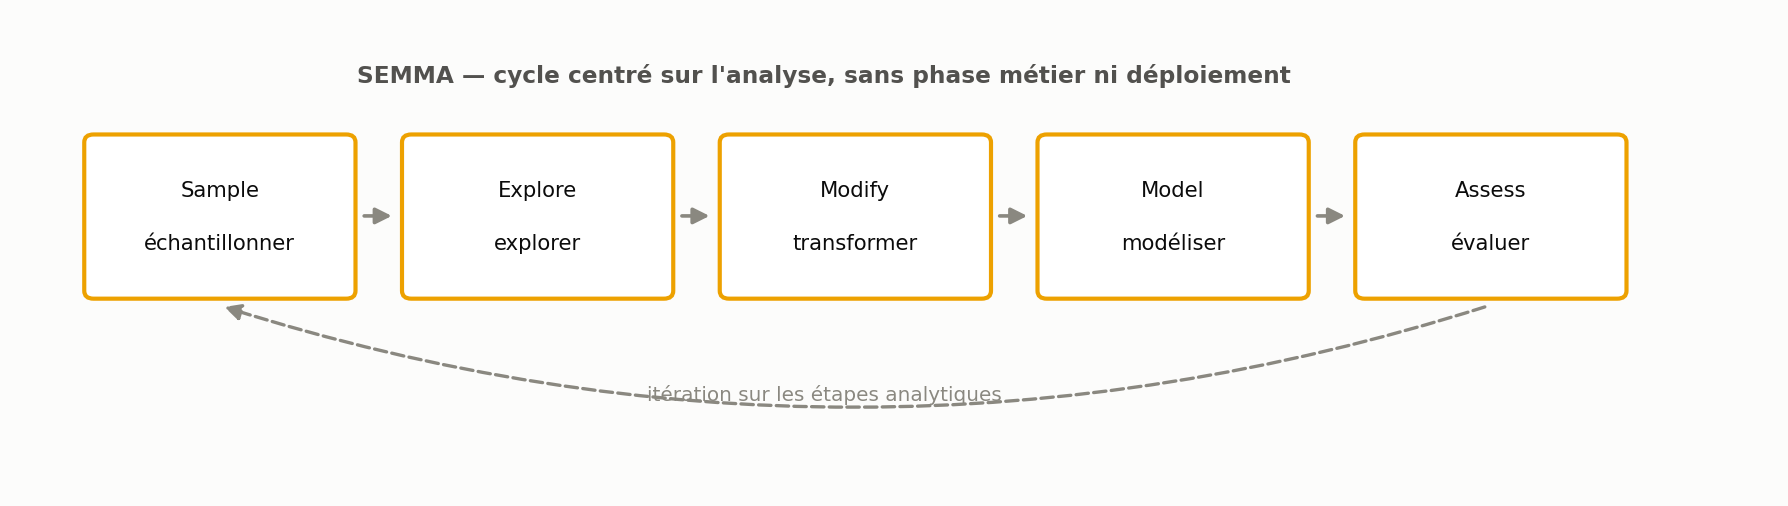
\includegraphics[width=0.88\textwidth]{img/semma_cycle.png}
    \caption{Cycle de vie de la méthodologie SEMMA}
    \label{fig:semma-cycle-chap1}
\end{figure}

\begin{enumerate}[label=\arabic*.]
    \item \textbf{Sample — Échantillonnage :} sélectionner un sous-ensemble représentatif des données disponibles afin de réduire le volume à traiter tout en conservant l'information utile.
    \item \textbf{Explore — Exploration :} examiner les données par des techniques statistiques et de visualisation afin d'identifier tendances, relations, anomalies et valeurs atypiques.
    \item \textbf{Modify — Modification :} nettoyer, transformer et enrichir les données ; sélectionner les variables pertinentes, en créer de nouvelles et traiter les valeurs manquantes.
    \item \textbf{Model — Modélisation :} construire les modèles statistiques ou d'apprentissage automatique adaptés à la problématique.
    \item \textbf{Assess — Évaluation :} mesurer la qualité et la performance des modèles afin de retenir la solution la plus pertinente.
\end{enumerate}

SEMMA est adaptée aux activités techniques de préparation et de modélisation, mais elle accorde peu de place à la compréhension métier, à la gestion de projet et au déploiement opérationnel.

% ------------------------------------------------------------
\subsection{Méthodologie KDD}
% ------------------------------------------------------------

KDD (\textit{Knowledge Discovery in Databases}) est une démarche de découverte de connaissances à partir de grands volumes de données, dont l'objectif est d'extraire des informations nouvelles, utiles et compréhensibles \cite{fayyad1996kdd}.

La figure~\ref{fig:kdd-cycle-chap1} en présente les étapes.

\begin{figure}[H]
    \centering
    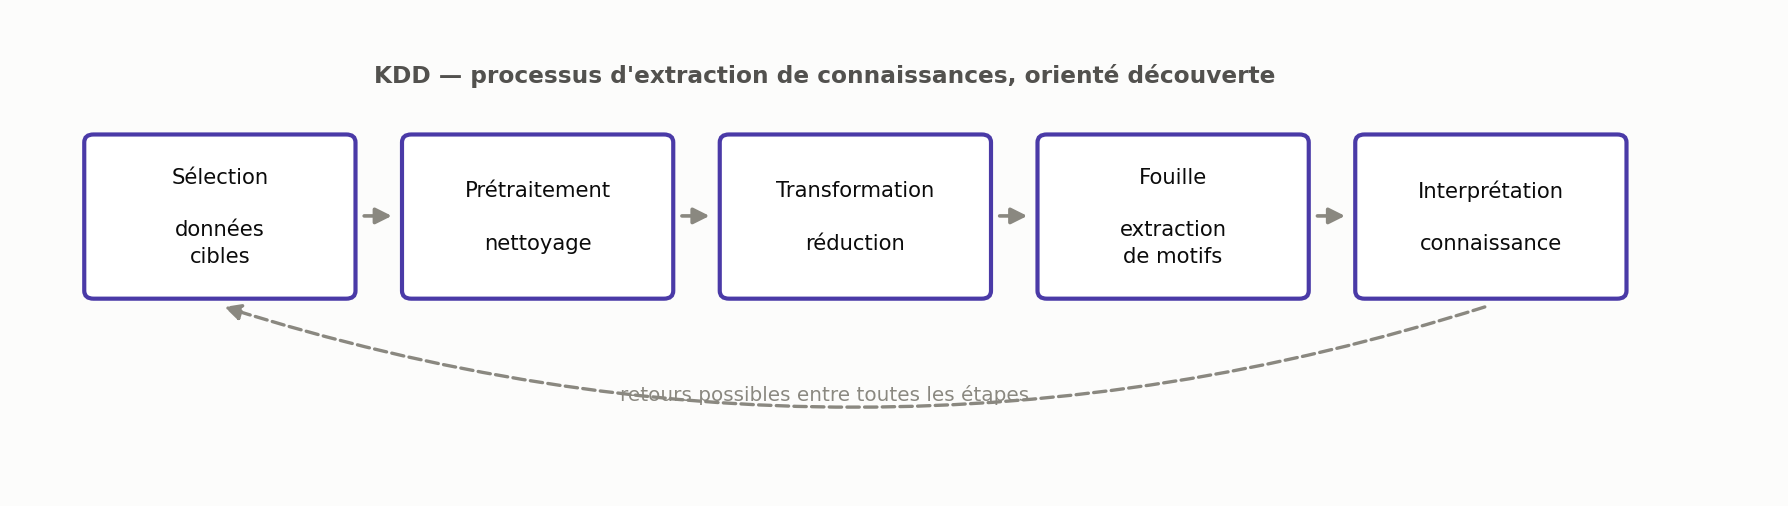
\includegraphics[width=0.92\textwidth]{img/kdd_cycle.png}
    \caption{Cycle de vie de la méthodologie KDD}
    \label{fig:kdd-cycle-chap1}
\end{figure}

\begin{enumerate}[label=\arabic*.]
    \item \textbf{Sélection des données :} identifier et extraire les données pertinentes au regard des objectifs.
    \item \textbf{Prétraitement :} nettoyer les données, corriger les incohérences, supprimer les doublons et traiter les valeurs manquantes.
    \item \textbf{Transformation :} normaliser, agréger, réduire la dimension et construire de nouvelles variables.
    \item \textbf{Data Mining :} appliquer des algorithmes statistiques ou d'apprentissage afin d'identifier des motifs et de produire des modèles.
    \item \textbf{Interprétation et évaluation :} analyser, valider et traduire les résultats sous une forme compréhensible par les parties prenantes.
\end{enumerate}

KDD constitue un cadre académique solide, mais elle détaille peu la gestion de projet, le développement applicatif, la collaboration avec les utilisateurs et le déploiement continu.

% ------------------------------------------------------------
\subsection{Méthodologie GIMSI}
% ------------------------------------------------------------

GIMSI \cite{fernandez2013gimsi} est une méthode de conception et de réalisation de systèmes d'aide à la décision. Elle vise à aligner les indicateurs de performance sur les objectifs stratégiques et opérationnels de l'organisation, en dix étapes regroupées en quatre phases.

La figure~\ref{fig:gimsi-cycle-chap1} en présente la démarche.

\begin{figure}[H]
    \centering
    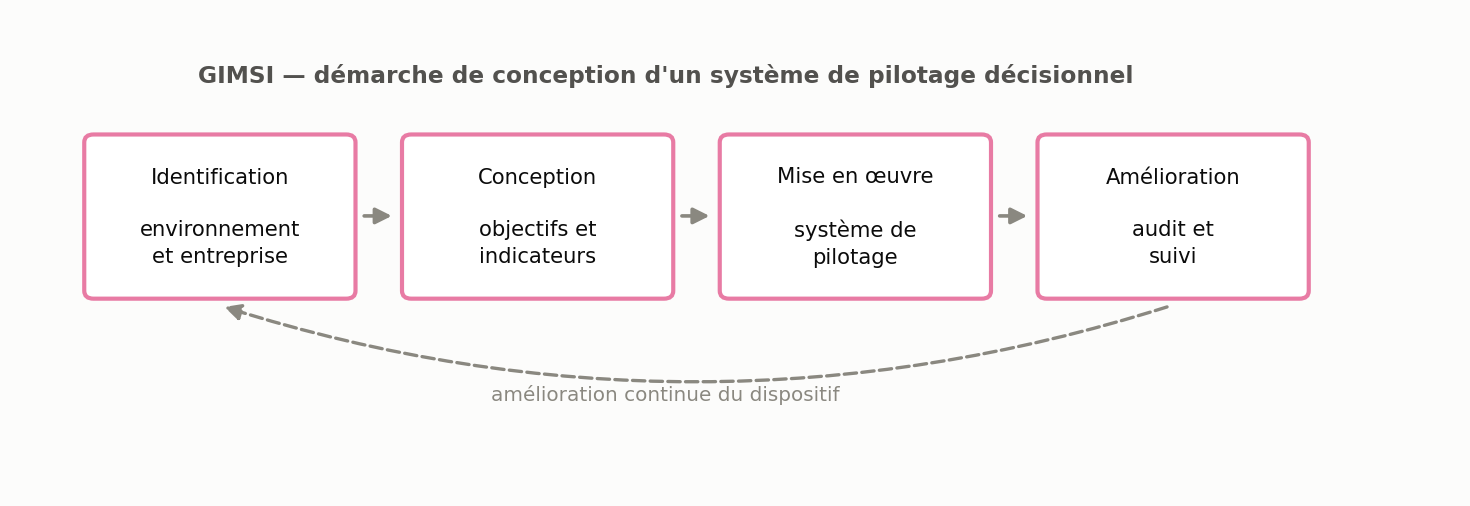
\includegraphics[width=0.78\textwidth]{img/gimsi_cycle.png}
    \caption{Cycle de vie de la méthodologie GIMSI}
    \label{fig:gimsi-cycle-chap1}
\end{figure}

\subsubsection*{Phase 1 : Identification}

\begin{enumerate}[label=\arabic*.]
    \item \textbf{Analyse de l'environnement :} étudier le contexte économique, la stratégie de l'entreprise et les enjeux du projet.
    \item \textbf{Analyse organisationnelle :} identifier les processus, les activités et les acteurs concernés par le système décisionnel.
\end{enumerate}

\subsubsection*{Phase 2 : Conception}

\begin{enumerate}[label=\arabic*.,start=3]
    \item \textbf{Définition des objectifs :} traduire les objectifs stratégiques en objectifs opérationnels mesurables.
    \item \textbf{Construction des tableaux de bord :} définir les vues nécessaires au pilotage des activités.
    \item \textbf{Choix des indicateurs :} sélectionner les indicateurs pertinents au regard des objectifs et des utilisateurs.
    \item \textbf{Collecte des informations :} identifier et collecter les données nécessaires au calcul des indicateurs.
    \item \textbf{Construction du système de pilotage :} organiser tableaux de bord et indicateurs en un système cohérent.
\end{enumerate}

\subsubsection*{Phase 3 : Mise en œuvre}

\begin{enumerate}[label=\arabic*.,start=8]
    \item \textbf{Choix des outils logiciels :} sélectionner les outils adaptés aux contraintes du projet.
    \item \textbf{Intégration et déploiement :} intégrer la solution au système d'information et la mettre à disposition des utilisateurs.
\end{enumerate}

\subsubsection*{Phase 4 : Amélioration permanente}

\begin{enumerate}[label=\arabic*.,start=10]
    \item \textbf{Audit et suivi :} évaluer régulièrement le système, mesurer son efficacité et proposer des améliorations.
\end{enumerate}

GIMSI est pertinente pour les projets décisionnels et la construction de tableaux de bord, mais elle est peu spécialisée dans la préparation des données, l'entraînement des modèles et l'organisation du développement logiciel.

% ------------------------------------------------------------
\subsection{Méthodologie CRISP-DM}
% ------------------------------------------------------------

CRISP-DM (\textit{Cross-Industry Standard Process for Data Mining}) \cite{chapman2000crisp,wirth2000crisp,shearer2000crisp} est l'une des méthodologies les plus utilisées pour conduire des projets de science des données, et le demeure vingt ans après sa publication \cite{martinez2021crisp,schroer2021systematic}. Elle fournit un cadre générique, structuré et itératif reliant les besoins métier aux activités de préparation des données, de modélisation, d'évaluation et de déploiement.

La figure~\ref{fig:crispdm-cycle-chap1} présente le cycle de vie de la méthode et ses six phases.

\begin{figure}[H]
    \centering
    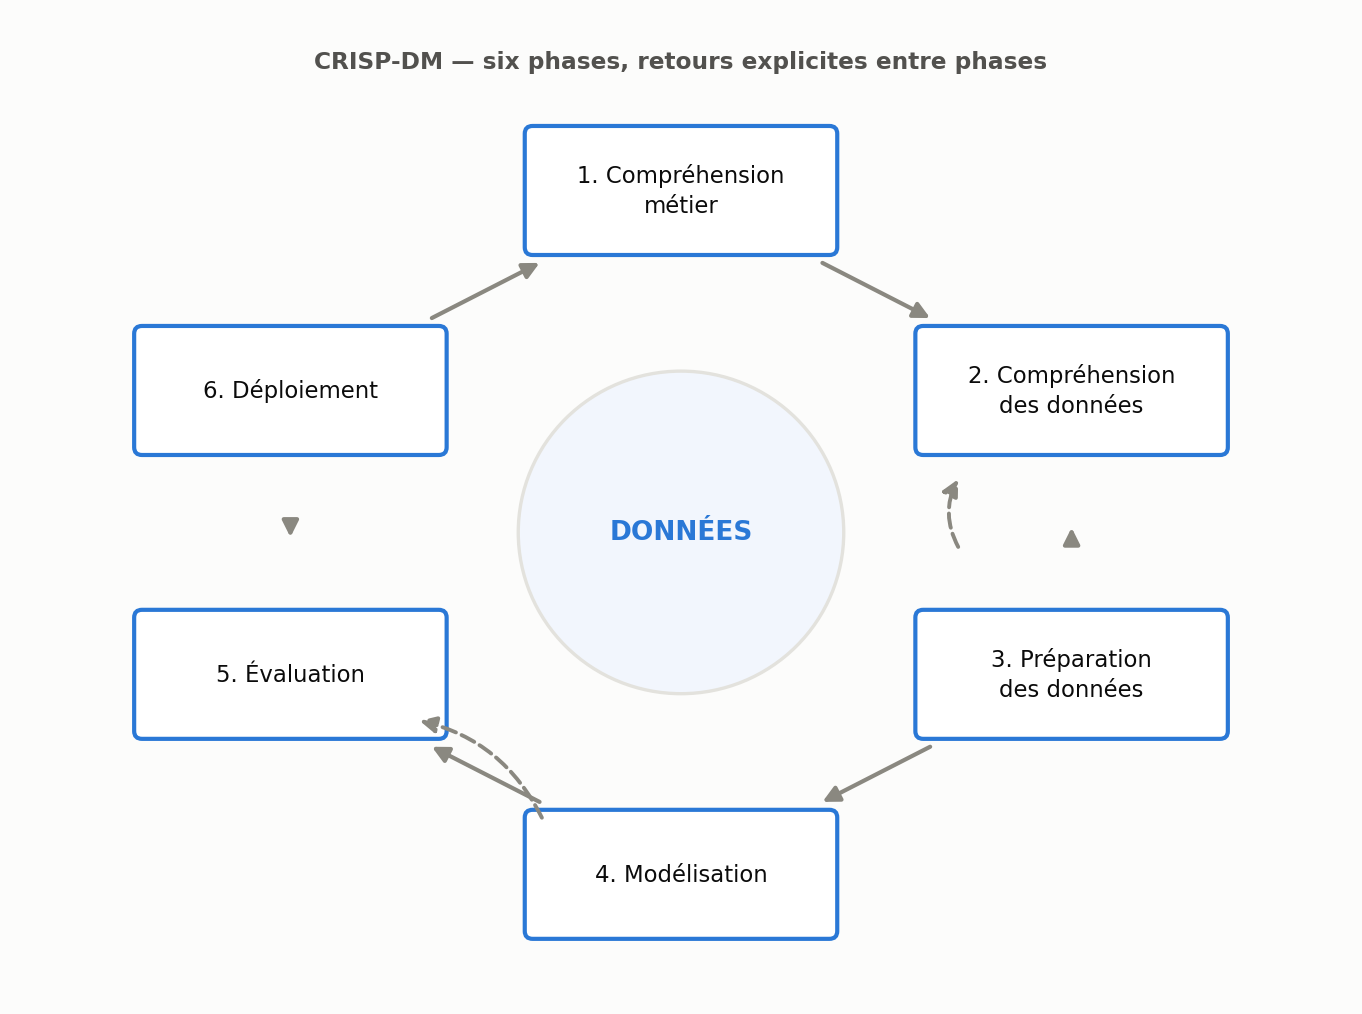
\includegraphics[width=0.78\textwidth]{img/crispdm_cycle.png}
    \caption{Cycle de vie de la méthodologie CRISP-DM}
    \label{fig:crispdm-cycle-chap1}
\end{figure}

\begin{enumerate}[label=\arabic*.]
    \item \textbf{Compréhension métier :} comprendre les objectifs de l'organisation, formaliser la problématique, identifier les contraintes et définir les critères de réussite.
    \item \textbf{Compréhension des données :} collecter les premières données, les décrire, les explorer et évaluer leur qualité.
    \item \textbf{Préparation des données :} nettoyer, sélectionner, transformer, intégrer et enrichir les données.
    \item \textbf{Modélisation :} sélectionner les techniques appropriées, entraîner les modèles et ajuster leurs paramètres.
    \item \textbf{Évaluation :} évaluer les modèles selon des métriques techniques et selon leur capacité à répondre aux objectifs métier.
    \item \textbf{Déploiement :} intégrer la solution validée dans un environnement opérationnel, la documenter, la suivre et la maintenir.
\end{enumerate}

CRISP-DM est particulièrement adaptée au projet : elle structure les activités liées aux données de vente et de stock, aux prévisions, à la détection des écarts et à l'évaluation des recommandations produites par les agents. Son caractère explicitement itératif constitue un atout majeur : les retours issus de l'évaluation ou du déploiement peuvent à tout moment ramener le projet vers la compréhension métier, la préparation des données ou la modélisation.

Processus générique et indépendant des technologies, CRISP-DM doit toutefois être instanciée pour un projet donné : elle ne fixe ni le découpage temporel du travail ni la manière de prioriser les fonctionnalités. Nous précisons plus loin comment ce cadre est appliqué sous la forme d'itérations successives, chacune produisant un incrément fonctionnel évaluable.

% ------------------------------------------------------------
\subsection{Méthodologie TDSP}
% ------------------------------------------------------------

Le \textit{Team Data Science Process} (TDSP) \cite{microsoft2020tdsp}, développé par Microsoft, organise les projets collaboratifs de science des données en combinant des pratiques issues de la data science, de l'ingénierie logicielle et des méthodes agiles.

La figure~\ref{fig:tdsp-cycle-chap1} en présente le cycle.

\begin{figure}[H]
    \centering
    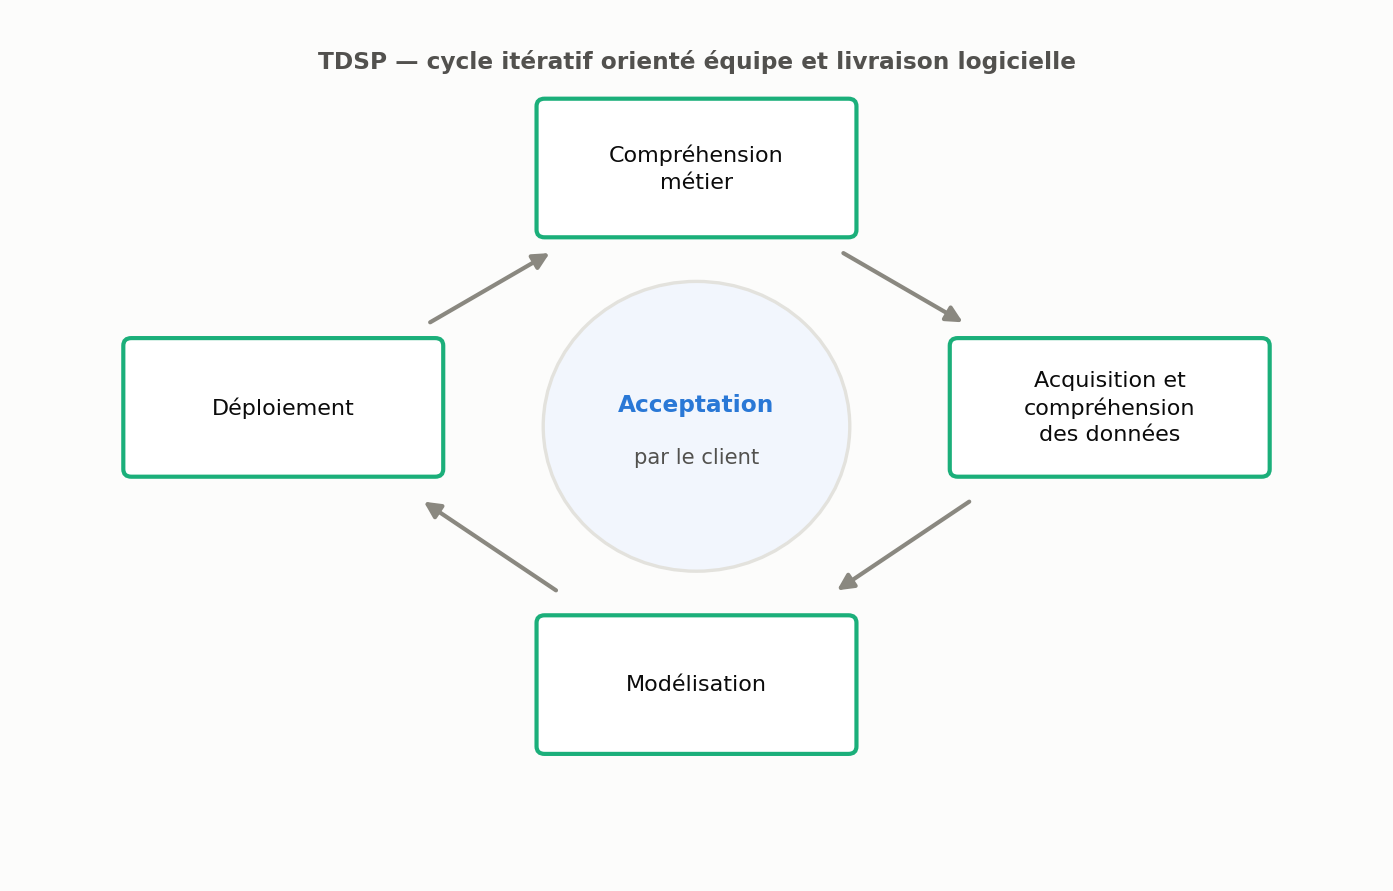
\includegraphics[width=0.90\textwidth]{img/tdsp_cycle.png}
    \caption{Cycle de vie de la méthodologie TDSP}
    \label{fig:tdsp-cycle-chap1}
\end{figure}

\begin{enumerate}[label=\arabic*.]
    \item \textbf{Compréhension métier :} définir les objectifs, les attentes des utilisateurs et les critères de réussite.
    \item \textbf{Acquisition et compréhension des données :} identifier, collecter, explorer et contrôler les sources de données.
    \item \textbf{Modélisation :} construire les variables, entraîner les modèles et analyser leurs performances.
    \item \textbf{Déploiement :} intégrer les modèles dans une application ou un environnement opérationnel.
    \item \textbf{Acceptation utilisateur :} faire valider la solution par les parties prenantes.
\end{enumerate}

TDSP précise également les rôles des membres d'une équipe data — architecte, chef de projet, ingénieur données, data scientist, développeur applicatif. Elle favorise l'industrialisation, mais reste relativement lourde pour un projet individuel et demeure historiquement liée à l'écosystème Microsoft.

% ------------------------------------------------------------
\subsection{Étude comparative des méthodologies}
% ------------------------------------------------------------

Le tableau~\ref{tab:comparaison-methodologies-chap1} présente une comparaison synthétique des méthodologies étudiées.

\begingroup
\setlength{\tabcolsep}{2pt}
\renewcommand{\arraystretch}{1.20}
\scriptsize

\begin{longtable}{|P{1.45cm}|P{1.80cm}|P{2.45cm}|P{2.60cm}|P{2.00cm}|P{1.85cm}|P{1.70cm}|}
\hline

\rowcolor{red!75}
\textcolor{white}{\textbf{Méthode}} &
\textcolor{white}{\textbf{Origine}} &
\textcolor{white}{\textbf{Étapes principales}} &
\textcolor{white}{\textbf{Caractéristiques}} &
\textcolor{white}{\textbf{Points forts}} &
\textcolor{white}{\textbf{Limites}} &
\textcolor{white}{\textbf{Orientation}} \\

\hline
\endfirsthead

\hline
\rowcolor{red!75}
\textcolor{white}{\textbf{Méthode}} &
\textcolor{white}{\textbf{Origine}} &
\textcolor{white}{\textbf{Étapes principales}} &
\textcolor{white}{\textbf{Caractéristiques}} &
\textcolor{white}{\textbf{Points forts}} &
\textcolor{white}{\textbf{Limites}} &
\textcolor{white}{\textbf{Orientation}} \\

\hline
\endhead

\hline
\endfoot

\hline
\endlastfoot

\textbf{SEMMA} &
SAS Institute &
Sample, Explore, Modify, Model, Assess &
Approche centrée sur l'analyse et la modélisation des données &
Simple, structurée, efficace pour l'expérimentation &
Compréhension métier et déploiement peu détaillés &
Data mining technique \\

\hline

\textbf{KDD} &
Recherche académique &
Sélection, prétraitement, transformation, data mining, interprétation &
Processus itératif de découverte de connaissances &
Fondement théorique solide, bonne structuration analytique &
Gestion de projet et déploiement peu détaillés &
Recherche et exploration \\

\hline

\textbf{GIMSI} &
Alain Fernandez &
Identification, conception, mise en œuvre, amélioration permanente &
Méthode coopérative centrée sur les systèmes décisionnels &
Bon alignement entre stratégie, objectifs et indicateurs &
Peu adaptée à la construction de modèles d'IA complexes &
Business Intelligence et pilotage \\

\hline

\textbf{CRISP-DM} &
Consortium industriel &
Compréhension métier, compréhension des données, préparation, modélisation, évaluation, déploiement &
Processus générique, itératif et indépendant des technologies &
Complet, adaptable, itératif, orienté valeur métier &
Générique : découpage temporel et priorisation à instancier &
Projets data et intelligence artificielle \\

\hline

\textbf{TDSP} &
Microsoft &
Compréhension métier, acquisition des données, modélisation, déploiement, acceptation utilisateur &
Approche collaborative orientée industrialisation &
Intègre data science, ingénierie logicielle et déploiement &
Plus lourde, fortement liée à l'écosystème Microsoft &
Data science en production \\

\hline

\caption{Tableau comparatif des méthodologies étudiées}
\label{tab:comparaison-methodologies-chap1}

\end{longtable}
\endgroup

% ------------------------------------------------------------
\subsection{Choix de la méthodologie adoptée}
% ------------------------------------------------------------

L'étude comparative montre que les méthodologies analysées ne présentent pas le même degré d'adéquation avec les besoins du projet.

SEMMA et KDD organisent efficacement les activités techniques de préparation et d'analyse, mais accordent peu de place à la compréhension métier, au développement applicatif et au déploiement progressif — trois dimensions centrales ici, puisque la solution doit être utilisée en boutique et pas seulement évaluée hors ligne.

GIMSI convient aux systèmes décisionnels et aux tableaux de bord, mais ne détaille pas suffisamment l'entraînement et l'évaluation des modèles, alors que le projet repose sur des prévisions dont la qualité doit être mesurée.

TDSP propose une démarche complète orientée industrialisation, mais suppose une équipe aux rôles clairement répartis et reste fortement associée à l'écosystème Microsoft, ce qui la rend peu adaptée au cadre d'un projet de fin d'études mené individuellement.

\textbf{CRISP-DM} est la méthodologie la plus adaptée pour encadrer l'ensemble du projet. Elle couvre la totalité du cycle de vie, de la compréhension du besoin métier jusqu'au déploiement, en passant par la compréhension des données, leur préparation, la modélisation et l'évaluation. Indépendante de toute technologie, elle s'applique aussi bien aux modèles de prévision qu'aux agents intelligents développés ici. Surtout, son caractère nativement itératif répond à la composante de développement logiciel : les phases ne sont pas parcourues une seule fois, mais réexécutées à chaque itération pour livrer des incréments successifs et intégrer les retours obtenus.

\textbf{La méthodologie adoptée est donc CRISP-DM}, appliquée de manière itérative et incrémentale. Ce choix unique évite la juxtaposition artificielle de deux cadres et conserve un fil conducteur cohérent, centré sur la donnée et sur la valeur métier, tout au long du rapport.

% ------------------------------------------------------------
\subsection{Instanciation de CRISP-DM au projet}
% ------------------------------------------------------------

CRISP-DM étant générique, il convient de préciser ce que chacune de ses phases recouvre concrètement dans ce projet. Le tableau~\ref{tab:instanciation-crispdm-chap1} établit cette correspondance.

\begin{longtable}{|P{3.0cm}|P{5.4cm}|P{5.6cm}|}
\hline
\rowcolor{red!75}
\textcolor{white}{\textbf{Phase CRISP-DM}} &
\textcolor{white}{\textbf{Activités menées}} &
\textcolor{white}{\textbf{Livrables correspondants}} \\
\hline
\endhead
\hline
\endfoot
\hline
\endlastfoot
Compréhension métier & Analyse du processus de vente en boutique, des rôles conseiller et manager, des objectifs commerciaux et des règles de réapprovisionnement & Périmètre, acteurs, besoins fonctionnels et non fonctionnels, backlog priorisé \\
\hline
Compréhension des données & Étude de l'historique de ventes journalier et horaire, des niveaux de stock, du catalogue produits, des objectifs et des signaux externes & Modèle de données, analyse de qualité et de couverture, identification des lacunes \\
\hline
Préparation des données & Construction du schéma versionné, nettoyage, calcul des variables calendaires et saisonnières, agrégations et vues métier & Base relationnelle multi-schémas, migrations, jeux de données d'entraînement \\
\hline
Modélisation & Moteur de séries temporelles pour les ventes, modèle de prévision de la demande, règles de gestion des stocks, agents intelligents et orchestration & Modèles de prévision, agents Ventes et Stocks, graphe d'orchestration \\
\hline
Évaluation & Backtests des prévisions, évaluation des recommandations par juge automatique, mesure du taux d'acceptation humaine, tests automatisés & Rapports de backtest, tableau de supervision de la qualité, suite de tests \\
\hline
Déploiement & Exposition des API, interfaces conseiller et manager, flux temps réel, conteneurisation et intégration continue & Application déployée, environnement conteneurisé, chaîne d'intégration \\
\hline
\caption{Instanciation des phases de CRISP-DM dans le projet}
\label{tab:instanciation-crispdm-chap1}
\end{longtable}

% ------------------------------------------------------------
\subsection{Application itérative de CRISP-DM}
% ------------------------------------------------------------

Dans l'approche retenue, les six phases ne sont pas exécutées une seule fois de manière strictement séquentielle. Elles sont parcourues au fil d'itérations successives et réexaminées dès que de nouvelles données, contraintes ou remarques métier apparaissent. Le projet est organisé en \textbf{douze itérations de deux semaines}, soit six mois : chaque itération se concentre sur un sous-ensemble de fonctionnalités et se termine par un incrément fonctionnel évaluable.

La compréhension métier initiale fixe le périmètre et les priorités. La compréhension et la préparation des données dominent les premières itérations. La modélisation et l'évaluation sont ensuite conduites de façon répétée, chaque modèle et chaque agent étant affiné à mesure des retours. Enfin, le déploiement, l'intégration et la stabilisation montent en importance dans les dernières itérations. La priorisation des fonctionnalités s'appuie sur la méthode \textbf{MoSCoW} (\textit{Must, Should, Could, Won't have}), qui distingue l'indispensable de l'accessoire ; le détail du backlog et de la planification est présenté au chapitre~\ref{chap:comprehension-metier}.

Le tableau~\ref{tab:iterations-crispdm-chap1} précise, pour chaque itération, la phase de CRISP-DM qui y domine.

\begin{longtable}{|P{2.30cm}|P{4.60cm}|P{6.20cm}|}
\hline

\rowcolor{red!75}
\textcolor{white}{\textbf{Itérations}} &
\textcolor{white}{\textbf{Phase CRISP-DM dominante}} &
\textcolor{white}{\textbf{Objectif principal}} \\

\hline
\endhead

\hline
\endfoot

\hline
\endlastfoot

It. 1 &
Compréhension métier et des données &
Cadrer le périmètre, analyser les sources de ventes et de stocks, poser les fondations techniques \\

\hline

It. 2 &
Préparation des données et modélisation &
Versionner le schéma, enrichir les variables saisonnières, construire le moteur de prévision et le premier tableau de bord \\

\hline

It. 3--4 &
Modélisation &
Développer l'assistant conversationnel, la base de connaissances métier et la robustesse des appels aux modèles de langage \\

\hline

It. 5--6 &
Modélisation et évaluation &
Enrichir le coaching (scores, substitution, contexte) et développer la supervision manager des ventes \\

\hline

It. 7--8 &
Préparation, modélisation et évaluation &
Traiter le domaine des stocks : état, analyse, prévision de demande et contraintes d'approvisionnement \\

\hline

It. 9--10 &
Modélisation, évaluation et déploiement &
Produire la décision de réapprovisionnement, orchestrer les agents et contrôler les réponses générées \\

\hline

It. 11--12 &
Déploiement et évaluation &
Valider par l'humain, ouvrir les flux temps réel, industrialiser et stabiliser la solution \\

\hline

\caption{Application des phases de CRISP-DM au fil des itérations du projet}
\label{tab:iterations-crispdm-chap1}
\end{longtable}

Cette organisation préserve le caractère itératif de CRISP-DM tout en assurant un suivi régulier, une priorisation explicite des besoins et une validation progressive des livrables. Chaque itération produit un résultat observable et contribue, pas à pas, à la construction du moteur agentique.

% ------------------------------------------------------------
\subsection{Correspondance entre les phases du cycle et le plan du rapport}
% ------------------------------------------------------------

Le choix de CRISP-DM n'a pas seulement gouverné la conduite du projet : il gouverne également la structure du présent document. La figure~\ref{fig:crispdm-chapitres-chap1} établit la correspondance entre chacune des six phases du cycle et le chapitre qui lui est consacré.

\begin{figure}[H]
    \centering
    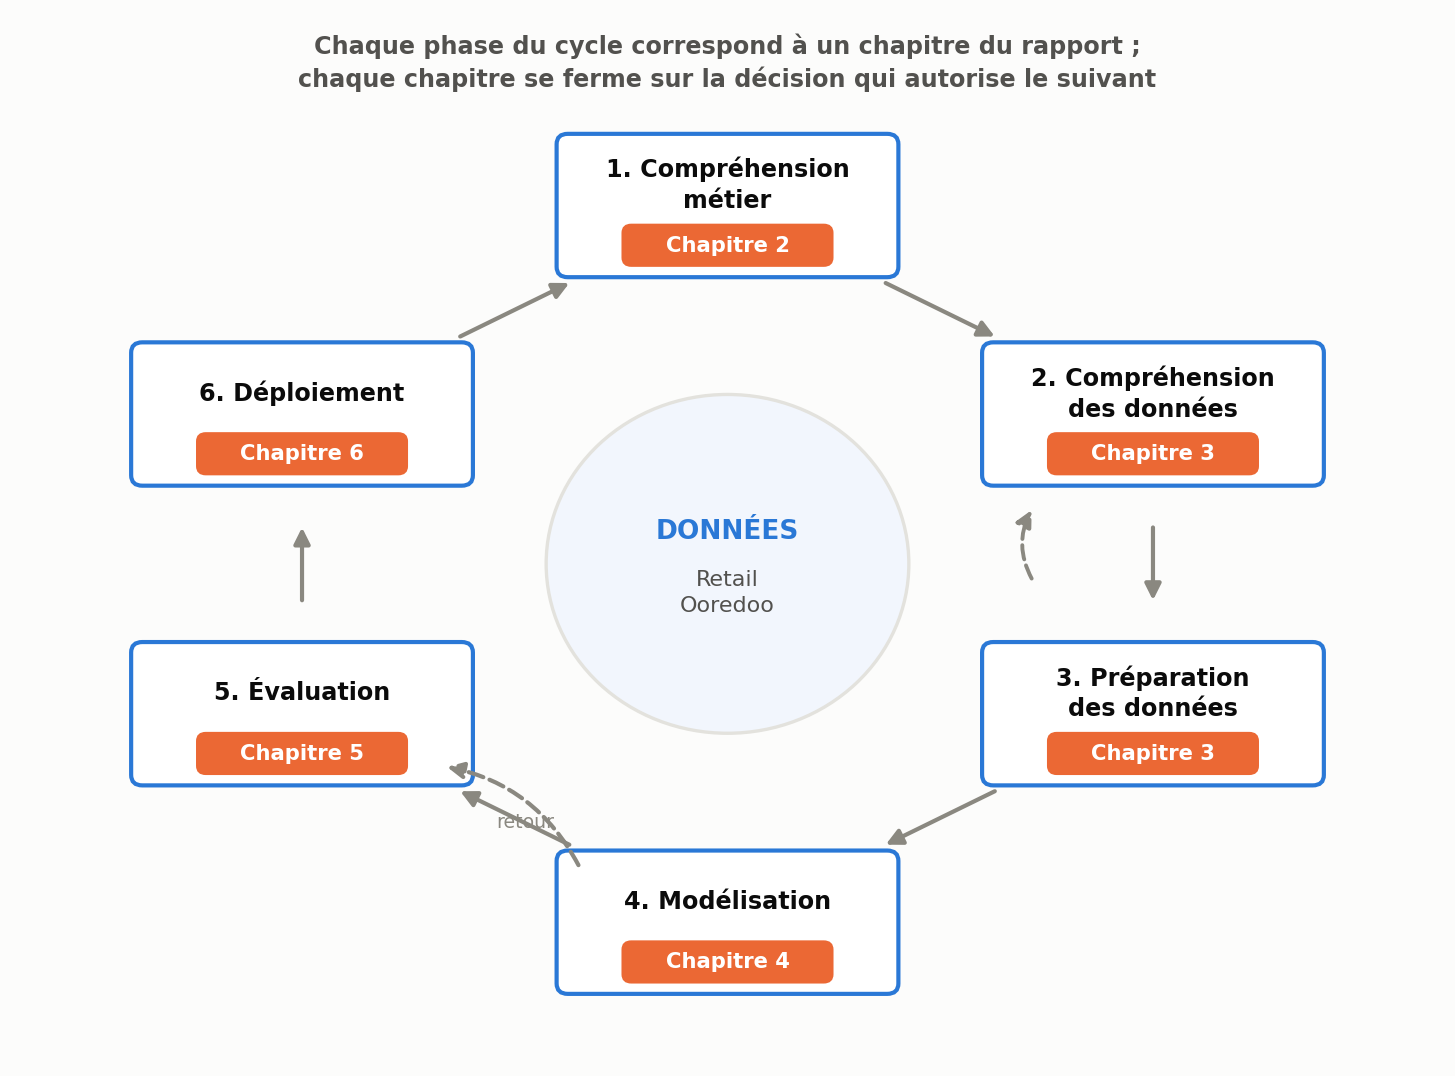
\includegraphics[width=0.82\textwidth]{img/fig_crispdm_chapitres.png}
    \caption{Correspondance entre les phases de CRISP-DM et les chapitres du rapport}
    \label{fig:crispdm-chapitres-chap1}
\end{figure}

Cette correspondance appelle deux précisions. D'une part, les phases 2 et 3 -- compréhension et préparation des données -- sont traitées dans un même chapitre : elles partagent les mêmes sources et s'entremêlent dans la pratique, une anomalie de qualité n'étant souvent découverte qu'en tentant de construire une variable. D'autre part, les phases 5 et 6 restent délibérément séparées, alors que de nombreux rapports les fusionnent en un chapitre unique de réalisation. L'évaluation constitue en effet le cœur scientifique de ce travail -- rétro-tests, juge automatique, retour humain -- et la subordonner à la présentation des interfaces l'affaiblirait.

Une convention est tenue tout au long du document : \textbf{chaque chapitre se ferme sur une décision explicite de fin de phase}, qui énonce ce que la phase a établi, sous quelles réserves, et ce qu'elle autorise. Cette convention est ce qui distingue un rapport \textit{conduit} par CRISP-DM d'un rapport qui se contente de citer la méthode en introduction.

% ------------------------------------------------------------
\subsection{Limites de CRISP-DM et compléments retenus}
% ------------------------------------------------------------

Aucune méthodologie n'est complète, et il serait malhonnête de présenter CRISP-DM sans en énoncer les angles morts. Trois d'entre eux concernent directement ce projet.

Le premier est que CRISP-DM \textbf{ne cadence pas la livraison d'un produit doté d'une interface utilisateur}. Le cycle décrit un processus d'analyse, non un processus de fabrication logicielle : il ne dit rien du rythme des livraisons, ni de la manière de présenter un incrément à un utilisateur. Ce manque est comblé par l'exécution itérative décrite ci-dessus -- douze itérations de deux semaines produisant chacune un incrément observable, avec une priorisation explicite du backlog. Il ne nécessite pas pour autant l'adoption d'un cadre agile formel : le projet étant mené par une personne seule, l'appareil cérémoniel de Scrum -- rôles distincts, réunions quotidiennes, revues formelles -- n'aurait apporté aucun bénéfice de coordination pour un coût réel de formalisme.

Le deuxième est que CRISP-DM, formalisé en 2000, \textbf{ne traite pas les spécificités des systèmes fondés sur des modèles génératifs} : non-déterminisme des sorties, évaluation de contenus textuels, dépendance à des services externes, garde-fous de conformité. Ces aspects appellent des dispositifs propres -- juge automatique, contrôles déterministes, cascade de repli -- qui sont introduits aux chapitres~\ref{chap:modelisation} et~\ref{chap:evaluation} en complément du cadre, et non contre lui.

Le troisième est que CRISP-DM \textbf{s'arrête au déploiement} et ne prescrit pas de dispositif de surveillance continue de la qualité en production. Or c'est précisément cette surveillance qui a révélé, au chapitre~\ref{chap:evaluation}, un écart substantiel entre la qualité mesurée en laboratoire et la qualité constatée en exploitation. Un dispositif de suivi permanent a donc été ajouté, décrit au chapitre~\ref{chap:deploiement}.

Ces trois compléments ne remettent pas en cause le choix de CRISP-DM : ils l'étendent là où il est muet, sans en altérer la structure ni la logique de progression.

% ------------------------------------------------------------
\section*{Conclusion}
\addcontentsline{toc}{section}{Conclusion}
% ------------------------------------------------------------

Ce chapitre a présenté le cadre général du projet. Nous avons introduit l'organisme d'accueil, Ooredoo Tunisie, ses activités, sa clientèle et son organisation, puis défini le cadre du projet, formulé la problématique et identifié les objectifs à atteindre.

L'étude de l'existant a mis en évidence les limites des approches classiques — reporting, CRM, Business Intelligence, planification des stocks et assistants génériques — lorsqu'elles sont employées séparément : vision fragmentée, faible actionnabilité, latence de la décision, absence de contextualisation, d'explicabilité et de garde-fous. Ces limites justifient une solution intégrée, capable d'exploiter les données Retail pour produire des recommandations actionnables, explicables, contrôlées et contextualisées.

Enfin, la méthodologie retenue est CRISP-DM, instanciée de manière itérative et incrémentale sur douze itérations de deux semaines, afin de concilier rigueur analytique et livraisons progressives. Son étude comparative avec SEMMA, KDD, GIMSI et TDSP a été conduite sur des critères explicites, et ses trois angles morts -- cadencement des livraisons, spécificités des systèmes génératifs, surveillance après déploiement -- ont été identifiés et assortis de compléments.

Cette base méthodologique sert de fil conducteur à la suite du rapport, dont chaque chapitre correspond désormais à une phase du cycle, conformément à la figure~\ref{fig:crispdm-chapitres-chap1}.

\textbf{Cadrage arrêté.} Le contexte, la problématique, le périmètre et la démarche sont fixés. Le chapitre suivant engage la première phase du cycle : la compréhension métier, qui traduira ce cadrage en objectifs mesurables.
